\documentclass[unnumsec,webpdf,modern,large]{mam-authoring-template}

\usepackage[utf8]{inputenc}
\usepackage[T1]{fontenc}
\usepackage[spanish]{babel}
\usepackage{booktabs}
\usepackage{tikz}
\usepackage{pgfplots}
\usepackage{amsmath}
\usepackage{graphicx}
\usepackage{array}
\usepackage{hyperref}
\usepackage{geometry}
\usepackage{subfigure}
\usepackage{biblatex}  % Ya lo tienes agregado
\addbibresource{ref.bib}  % El archivo .bib

\graphicspath{{Fig/}}

\theoremstyle{thmstyleone}%
\newtheorem{theorem}{Teorema}%
\newtheorem{proposition}[theorem]{Proposición}%
\theoremstyle{thmstyletwo}%
\newtheorem{example}{Ejemplo}%
\newtheorem{remark}{Observación}%
\theoremstyle{thmstylethree}%
\newtheorem{definition}{Definición}

\begin{document}

\journaltitle{Informe Científico}
\DOI{...}
\copyrightyear{2025}
\pubyear{2025}
\access{Publicación Anticipada: 17 de febrero de 2025}

\firstpage{1}
\title{Comparación de Imágenes Generadas por IA Utilizando Características SIFT y ORB}

\author[1]{Agnelly Sañay Cabrera}
\author[2]{Justin Tobar Soberon}
\author[3]{Angel Pozo Benavidez}

\authormark{Sañay, Tobar, Pozo}

\address[1]{\orgdiv{Ciencias de la Computación}, \orgname{Universidad Politécnica Salesiana}}

\abstract{Este trabajo compara generadores de imágenes utilizando descriptores SIFT y ORB en tres Modelos de IA: BING, DALL-E y LEONARDO. Se aplicaron procesos de reprocesamiento como redimensionamiento y suavizado, y se evaluaron mediante distancias euclidianas y hamming. Los resultados indican que LEONARDO y DALL-E lograron un número similar de coincidencias, mientras que BING presentó un rendimiento inferior. Los tiempos de ejecución fueron mínimos en todos los casos, demostrando que la IA puede procesar imágenes en español e inglés de manera consistente.}

\keywords{Generación de imágenes, descriptores SIFT, descriptores ORB, BING, DALL-E, LEONARDO, procesamiento multilingüe}

\maketitle

\section{Introducción}
En el presente trabajo se aborda el análisis comparativo de imágenes generadas por inteligencia artificial a partir de prompts en inglés y español. Para llevar a cabo este estudio, se accede al repositorio de GitHub: \cite{hustler013_comparacion_2025} , donde se encuentran disponibles los prompts y las imágenes generadas en tres herramientas distintas. El proceso consiste en extraer las características SIFT (Scale-Invariant Feature Transform) y ORB (Oriented FAST and Rotated BRIEF) de cada una de las imágenes generadas, con el objetivo de analizar sus similitudes y diferencias.

Una vez extraídas las características, se procede a comparar cada imagen generada con su prompt en inglés con su correspondiente imagen generada con el prompt en español. La comparación se realiza mediante el cálculo de distancias, empleando la distancia euclidiana para las características SIFT y la distancia de Hamming para las características ORB. Este enfoque permite evaluar la consistencia y variabilidad en las imágenes generadas por IA al cambiar el idioma del prompt \cite{castro2025_comparacion}.


\section{Metodología}
\subsection{BING}
El proceso de análisis comenzó con la recolección de un conjunto de imágenes normalizadas, que se almacenaron en los directorios \texttt{norm\_esp\_dir} y \texttt{norm\_eng\_dir}. Se utilizó la librería OpenCV (cv2) para la lectura de las imágenes desde estos directorios. A través del uso de IA BING, se realizó un análisis de las imágenes normalizadas, considerando las siguientes etapas:

\begin{enumerate}
    \item \textbf{Montaje de Google Drive y Carga de Imágenes:} Se montó Google Drive para acceder a los directorios que contienen las imágenes en los idiomas Español e Inglés. Las imágenes fueron cargadas desde las rutas \texttt{esp\_dir} y \texttt{eng\_dir}, y se verificó que ambas carpetas contenían la misma cantidad de imágenes.
    
    \item  \textbf{Preprocesamiento de Imágenes:} Las imágenes fueron preprocesadas antes de someterlas al análisis. Este paso incluyó:
    \begin{itemize}
        \item Redimensionado de las imágenes a un tamaño uniforme de 256x256 píxeles.
        \item Conversión de las imágenes a escala de grises para facilitar la extracción de características.
        \item Suavizado Gaussiano para reducir el ruido y mejorar la precisión de la detección de características.
        \item Normalización de las imágenes para asegurar que los valores de los píxeles estén en el rango [0, 1].
    \end{itemize}
    
    \item \textbf{Extracción de Características:} Se aplicaron dos algoritmos para la extracción de características clave de las imágenes preprocesadas:
    \begin{itemize}
        \item \textbf{SIFT (Scale-Invariant Feature Transform)}: Este algoritmo fue utilizado para detectar y describir características invariantes a escala y rotación en las imágenes.
        \item \textbf{ORB (Oriented FAST and Rotated BRIEF)}: Se utilizó como alternativa más eficiente, especialmente en entornos con limitaciones de procesamiento.
    \end{itemize}
    
    \item \textbf{Normalización de Descriptores:} Los descriptores extraídos con SIFT y ORB fueron normalizados para asegurar que sus valores estuvieran en el rango [0, 1], lo cual mejora la comparación y precisión en el análisis.

    \item \textbf{Comparación de Descriptores:} Se calcularon las distancias y coincidencias entre los descriptores extraídos de las imágenes utilizando dos métodos de comparación:
    \begin{itemize}
        \item \textbf{Distancia Euclidiana:} Se utilizó para comparar los descriptores extraídos con SIFT, utilizando el descriptor \texttt{cv2.NORM\_L2}.
        \item \textbf{Distancia Hamming:} Se utilizó para comparar los descriptores extraídos con ORB, utilizando el descriptor \texttt{cv2.NORM\_HAMMING}.
    \end{itemize}

    \begin{figure}[h]
    \centering
    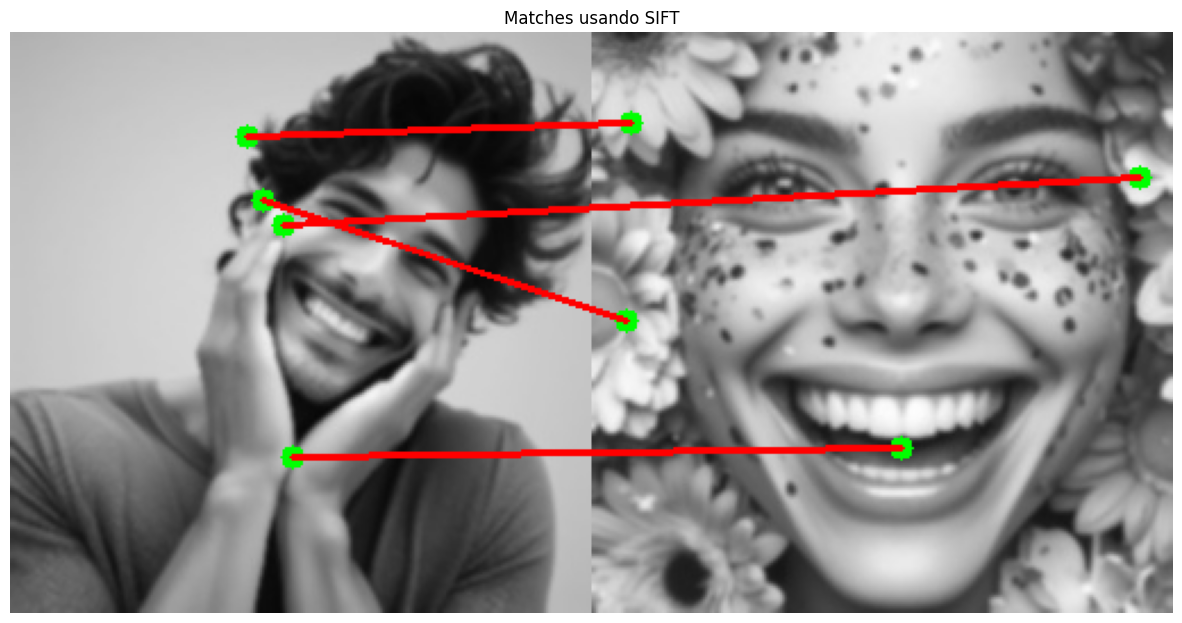
\includegraphics[width=0.5\textwidth]{bing1.png}
    \caption{Comparacion entre imagenes generadas por promp de Español e Ingles}
    \label{fig:mesh1}
    \end{figure}

    \begin{figure}[h]
    \centering
    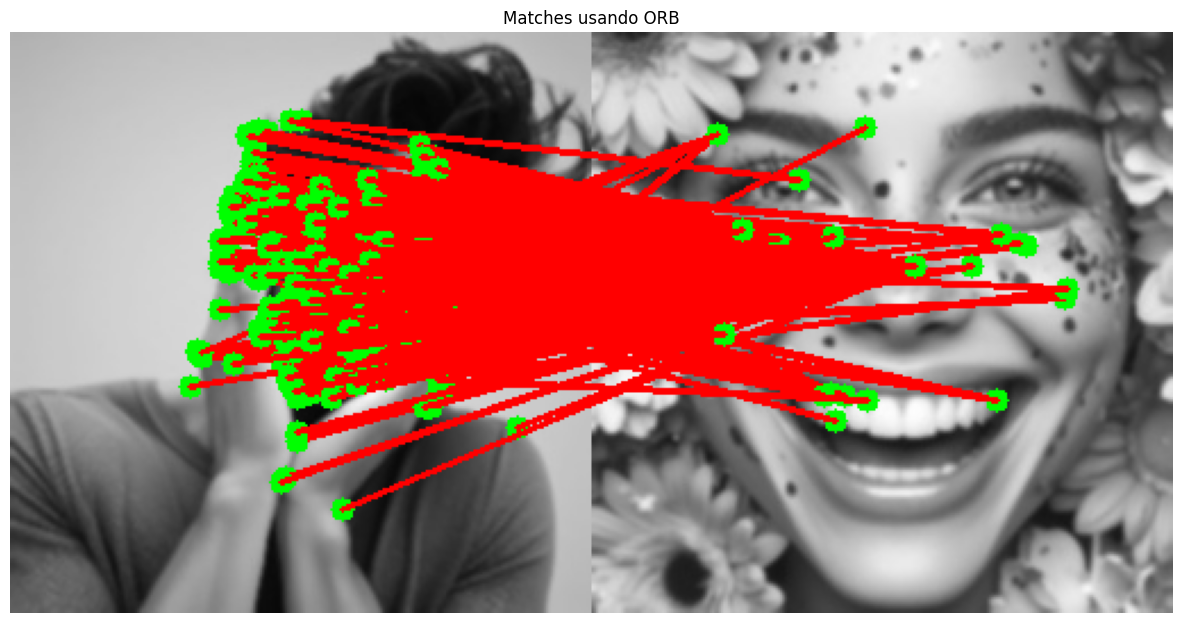
\includegraphics[width=0.5\textwidth]{bing2.png}
    \caption{Comparacion entre imagenes generadas por promp de Español e Ingles}
    \label{fig:mesh1}
    \end{figure}

    \item \textbf{Evaluación de Resultados:} Los resultados fueron evaluados en términos de precisión y eficiencia. Se analizaron las siguientes métricas:
    \begin{itemize}
        \item \textbf{Número de Coincidencias:} Se calculó la cantidad promedio de coincidencias entre las características extraídas de las imágenes en español e inglés.
        \item \textbf{Tiempo de Extracción de Características:} Se evaluó el tiempo promedio necesario para extraer características de las imágenes.
        \item \textbf{Distancia Media:} Se evaluaron las distancias promedio entre las características extraídas de las imágenes en español e inglés.
    \end{itemize}
\end{enumerate}

\subsection{DALL-E}
El proceso de análisis comenzó con la recolección de un conjunto de imágenes normalizadas, las cuales fueron almacenadas en los directorios \texttt{norm\_esp\_dir} y \texttt{norm\_eng\_dir}. Se utilizó la librería OpenCV (\texttt{cv2}) para leer las imágenes desde estos directorios. A través de la IA DALL-E, se llevó a cabo un análisis de las imágenes normalizadas, considerando las siguientes etapas:

\begin{enumerate}
    \item \textbf{Montaje de Google Drive y Carga de Imágenes:} Se montó Google Drive para acceder a los directorios que contienen las imágenes en los idiomas español e inglés. Las imágenes fueron cargadas desde las rutas \texttt{esp\_dir} y \texttt{eng\_dir}, y se verificó que ambas carpetas contenían la misma cantidad de imágenes.

    El proceso de normalización consistió en ajustar las dimensiones y resoluciones de las imágenes generadas, asegurando una comparación objetiva entre los diferentes resultados. Esto fue fundamental para evaluar cómo la IA era capaz de reproducir los elementos solicitados en las descripciones.

    \item \textbf{Preprocesamiento de Imágenes:} Las imágenes fueron preprocesadas antes de someterlas al análisis. Este paso incluyó:
    \begin{itemize}
        \item Redimensionado de las imágenes a un tamaño uniforme de 256x256 píxeles.
        \item Conversión de las imágenes a escala de grises para facilitar la extracción de características.
        \item Suavizado Gaussiano para reducir el ruido y mejorar la precisión en la detección de características.
        \item Normalización de las imágenes para asegurar que los valores de los píxeles estén en el rango [0, 1].
    \end{itemize}

    \item \textbf{Extracción de Características:} Se aplicaron dos algoritmos para la extracción de características clave de las imágenes preprocesadas:
    \begin{itemize}
        \item \textbf{SIFT (Scale-Invariant Feature Transform):} Este algoritmo se utilizó para detectar y describir características invariantes a escala y rotación en las imágenes.
        \item \textbf{ORB (Oriented FAST and Rotated BRIEF):} Se utilizó como alternativa más eficiente, especialmente en entornos con limitaciones de procesamiento.
    \end{itemize}

    \item \textbf{Normalización de Descriptores:} Los descriptores extraídos con SIFT y ORB fueron normalizados para asegurar que sus valores estuvieran en el rango [0, 1], lo cual mejora la comparación y precisión en el análisis.

    \item \textbf{Comparación de Descriptores:} Se calcularon las distancias y coincidencias entre los descriptores extraídos de las imágenes utilizando dos métodos de comparación:
    \begin{itemize}
        \item \textbf{Distancia Euclidiana:} Se utilizó para comparar los descriptores extraídos con SIFT, utilizando el descriptor \texttt{cv2.NORM\_L2}.
        \item \textbf{Distancia Hamming:} Se utilizó para comparar los descriptores extraídos con ORB, utilizando el descriptor \texttt{cv2.NORM\_HAMMING}.
    \end{itemize}
    \begin{figure}[h]
    \centering
    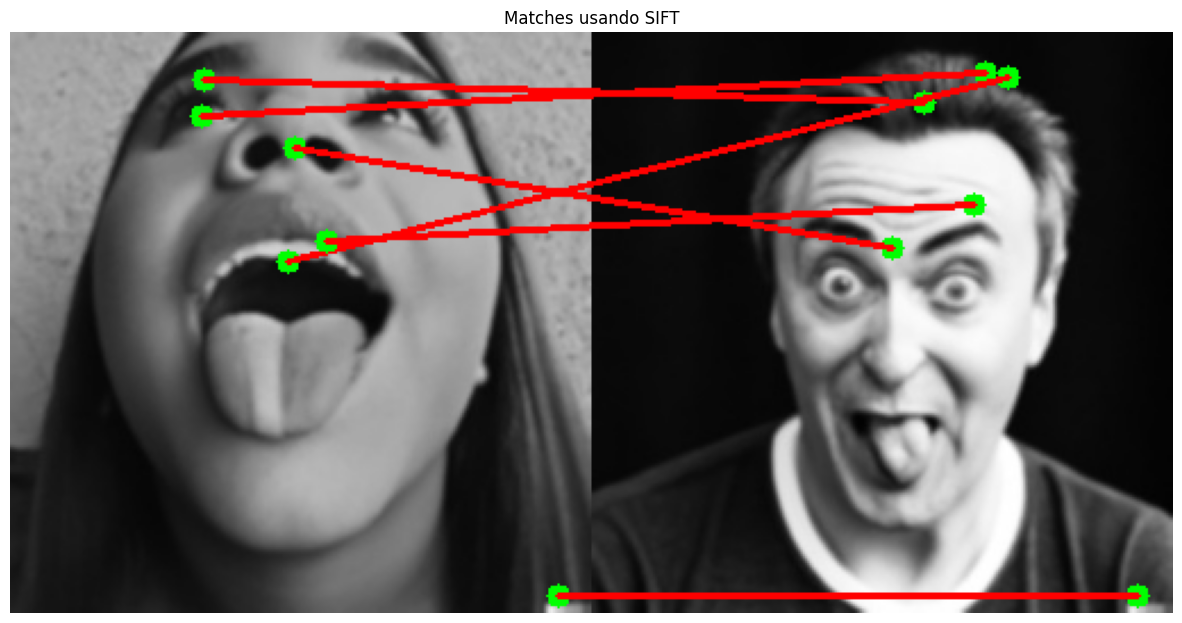
\includegraphics[width=0.5\textwidth]{dalle1.png}
    \caption{Comparacion entre imagenes generadas por promp de Español e Ingles}
    \label{fig:mesh1}
    \end{figure}

    \begin{figure}[h]
    \centering
    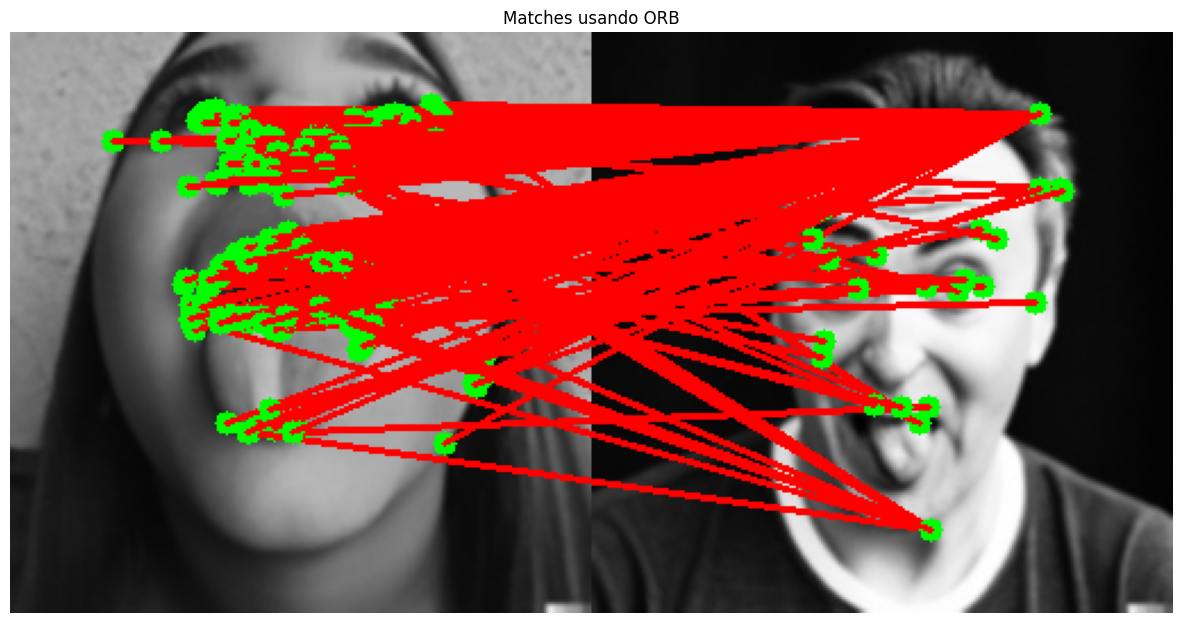
\includegraphics[width=0.5\textwidth]{dalle2.png}
    \caption{Comparacion entre imagenes generadas por promp de Español e Ingles}
    \label{fig:mesh1}
    \end{figure}
\end{enumerate}

\subsection{LEONARDO}  
El proceso de análisis se llevó a cabo utilizando la IA LEONARDO, diseñada para comparar imágenes en español e inglés mediante la extracción y comparación de características. Se utilizaron descriptores SIFT y ORB, evaluando distancias euclideanas y Hamming, así como el análisis de coincidencias y tiempos de extracción. El flujo de trabajo siguió las siguientes etapas:

\begin{enumerate}
    \item \textbf{Montaje de Google Drive y Carga de Imágenes:} Se montó Google Drive para acceder a los directorios que contienen las imágenes en los idiomas Español e Inglés. Las imágenes fueron cargadas desde las rutas \texttt{norm\_esp\_dir} y \texttt{norm\_eng\_dir} utilizando la librería OpenCV (\texttt{cv2.imread}), asegurando que ambas carpetas contenían la misma cantidad de imágenes.

    \item \textbf{Normalización de Imágenes:} Para garantizar consistencia en el análisis, las imágenes fueron normalizadas siguiendo estos pasos:
    \begin{itemize}
        \item Redimensionado a 256x256 píxeles para un tamaño uniforme.
        \item Conversión a escala de grises, optimizando la extracción de características.
        \item Aplicación de Suavizado Gaussiano para reducir el ruido.
    \end{itemize}
    Las imágenes normalizadas se almacenaron en los directorios \texttt{norm\_esp} y \texttt{norm\_eng}.

    \item \textbf{Extracción de Características:} Se emplearon dos algoritmos clave para la extracción de características:
    \begin{itemize}
        \item \textbf{SIFT (Scale-Invariant Feature Transform):} Utilizado para detectar y describir características invariantes a escala y rotación, proporcionando descriptores robustos para la comparación.
        \item \textbf{ORB (Oriented FAST and Rotated BRIEF):} Seleccionado por su eficiencia computacional, especialmente útil en entornos con limitaciones de procesamiento.
    \end{itemize}
    
    \item \textbf{Normalización de Descriptores:} Los descriptores extraídos con SIFT y ORB fueron normalizados al rango [0, 1], utilizando técnicas de normalización de \texttt{scikit-learn}, mejorando así la precisión en las comparaciones.

    \item \textbf{Comparación de Descriptores:} Se utilizó el método \texttt{match\_descriptors} de \texttt{skimage} para comparar las características entre las imágenes en español e inglés, aplicando las siguientes métricas:
    \begin{itemize}
        \item \textbf{Distancia Euclidiana:} Utilizada para comparar los descriptores SIFT, permitiendo evaluar la similitud basada en la magnitud de las diferencias.
        \item \textbf{Distancia Hamming:} Aplicada para los descriptores ORB, ideal para comparaciones binarias de alta eficiencia.
    \end{itemize}

    \begin{figure}[h]
    \centering
    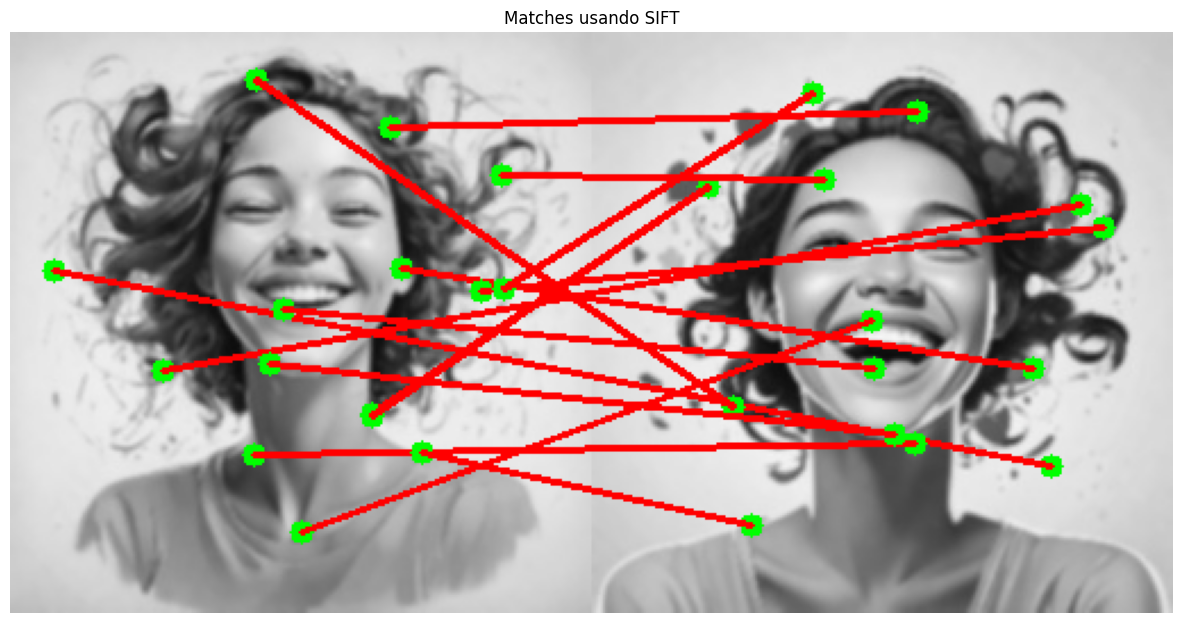
\includegraphics[width=0.5\textwidth]{leo1.png}
    \caption{Comparacion entre imagenes generadas por promp de Español e Ingles}
    \label{fig:mesh1}
    \end{figure}

    \begin{figure}[h]
    \centering
    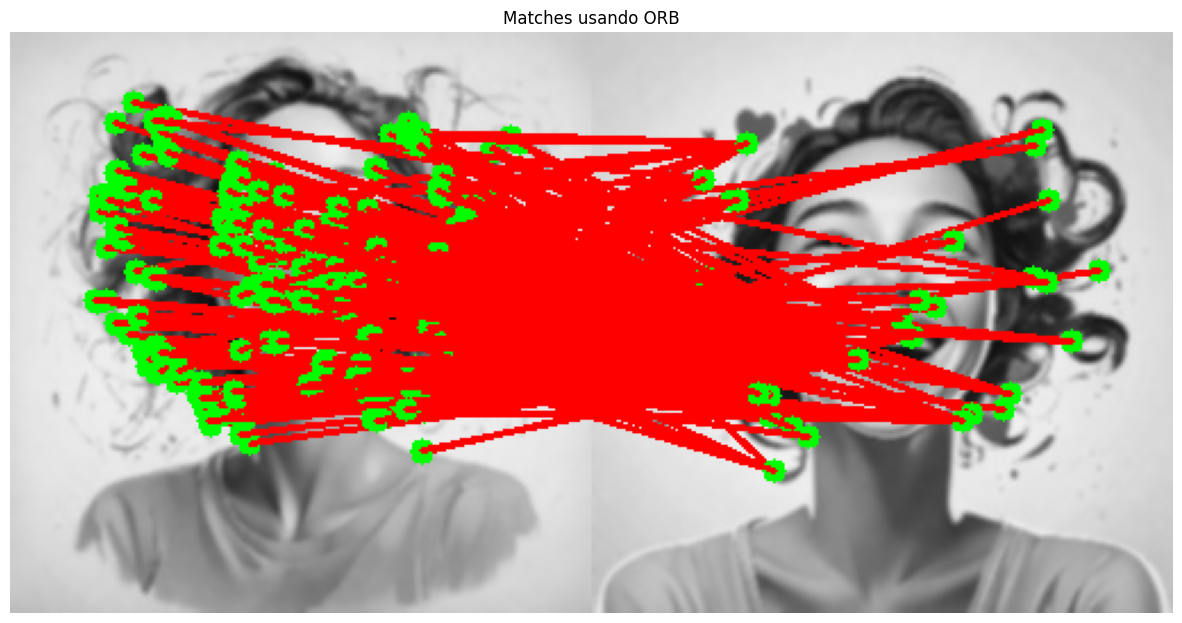
\includegraphics[width=0.5\textwidth]{leo2.png}
    \caption{Comparacion entre imagenes generadas por promp de Español e Ingles}
    \label{fig:mesh1}
    \end{figure}

    \item \textbf{Evaluación de Resultados:} Se analizaron las siguientes métricas para evaluar la precisión y eficiencia del proceso:
    \begin{itemize}
        \item \textbf{Número de Coincidencias:} Se calculó el número promedio de coincidencias entre las imágenes en ambos idiomas.
        \item \textbf{Tiempo de Extracción de Características:} Se midió el tiempo promedio requerido para extraer características con SIFT y ORB.
        \item \textbf{Distancia Media:} Se evaluaron las distancias promedio (Euclidiana para SIFT y Hamming para ORB) entre las características extraídas.
        \item \textbf{Desviación Estándar:} Se calculó la dispersión de las distancias, proporcionando información sobre la consistencia de las coincidencias.
    \end{itemize}

    \item \textbf{Exportación de Resultados:} Los resultados fueron almacenados en un archivo CSV denominado \texttt{LEONARDO.csv}, el cual incluye detalles de las coincidencias y estadísticas de comparación, facilitando análisis cuantitativos y cualitativos posteriores.
\end{enumerate}


\section{Resultados}
\subsection{BING}
A continuación, se presentan los resultados obtenidos a partir del análisis de las imágenes utilizando las técnicas de extracción de características SIFT y ORB. Los resultados incluyen métricas sobre las coincidencias, tiempos de extracción de características, número de características extraídas y distancias entre descriptores.

\subsubsection{Métricas SIFT}

Las métricas obtenidas para la técnica SIFT son las siguientes:

\begin{center}
\begin{tabular}{ | m{7em} | m{1.5cm} | m{1.5cm} | } 
  \hline
  \textbf{Métrica} & \textbf{Valor} & \textbf{Desviación Estándar} \\ 
  \hline
  Coincidencias (min) & 0 & - \\ 
  \hline
  Coincidencias (máx) & 57 & - \\ 
  \hline
  Coincidencias (promedio) & 11.94 & 9.76 \\ 
  \hline
  Tiempo (min) & 0.0258 s & - \\ 
  \hline
  Tiempo (máx) & 0.1281 s & - \\ 
  \hline
  Tiempo (promedio) & 0.0635 s & 0.0225 s \\ 
  \hline
  Características (min) & 44 & - \\ 
  \hline
  Características (máx) & 502 & - \\ 
  \hline
  Características (promedio) & 382.12 & 147.68 \\ 
  \hline
  Distancia (min) & 0.5145 & - \\ 
  \hline
  Distancia (máx) & 2.0433 & - \\ 
  \hline
  Distancia (promedio) & 1.3475 & 0.2480 \\ 
  \hline
\end{tabular}
\end{center}

\subsubsection{Métricas ORB}

Las métricas obtenidas para la técnica ORB son las siguientes:

\begin{center}
\begin{tabular}{ | m{7em} | m{1.5cm} | m{1.5cm} | } 
  \hline
  \textbf{Métrica} & \textbf{Valor} & \textbf{Desviación Estándar} \\ 
  \hline
  Coincidencias (min) & 47 & - \\ 
  \hline
  Coincidencias (máx) & 454 & - \\ 
  \hline
  Coincidencias (promedio) & 393.72 & 73.50 \\ 
  \hline
  Tiempo (min) & 0.0029 s & - \\ 
  \hline
  Tiempo (máx) & 0.0154 s & - \\ 
  \hline
  Tiempo (promedio) & 0.0075 s & 0.0024 s \\ 
  \hline
  Características (min) & 56 & - \\ 
  \hline
  Características (máx) & 474 & - \\ 
  \hline
  Características (promedio) & 421.85 & 71.13 \\ 
  \hline
  Distancia (min) & 0.8330 & - \\ 
  \hline
  Distancia (máx) & 3.3436 & - \\ 
  \hline
  Distancia (promedio) & 2.2121 & 0.3202 \\ 
  \hline
\end{tabular}
\end{center}


\subsubsection{Cantidad de Matches}
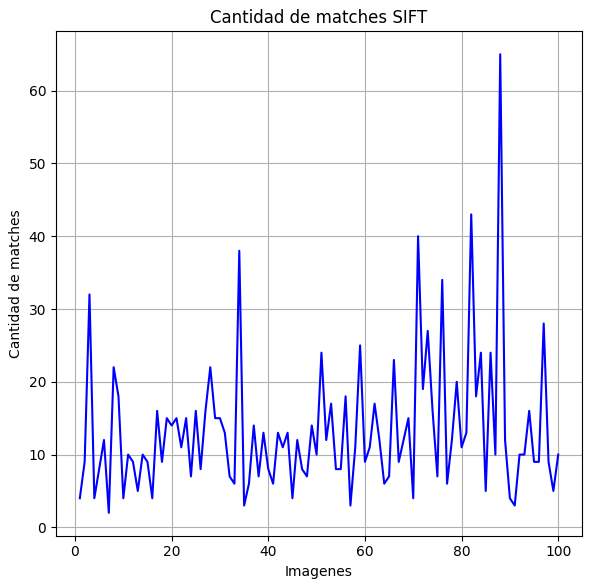
\includegraphics[width=7cm]{1.png}
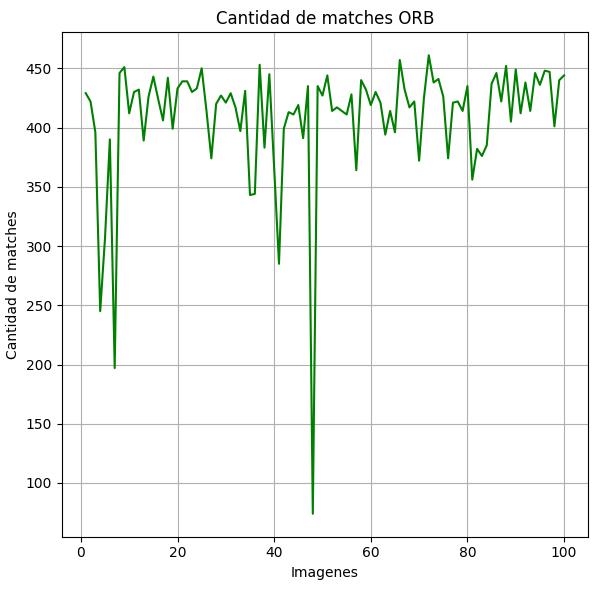
\includegraphics[width=7cm]{1.1.1.png}

\subsubsection{Distancias Promedio de los descriptores}
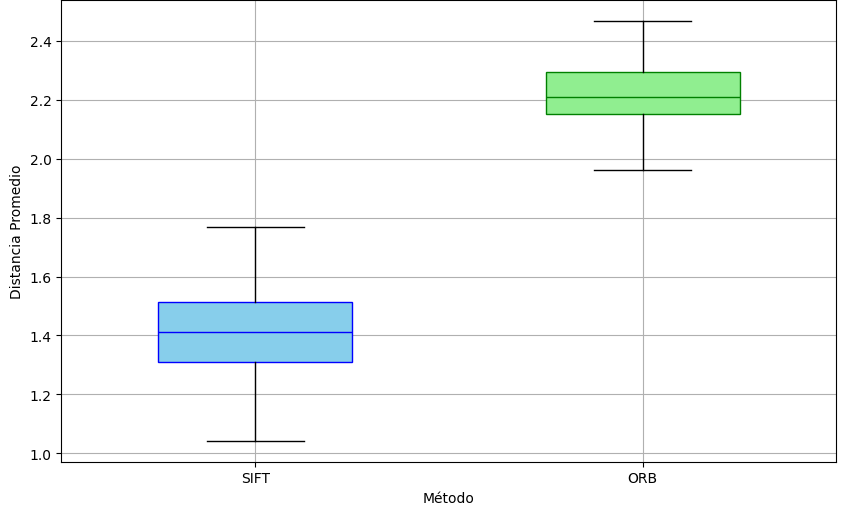
\includegraphics[width=6.5cm]{1.1.2.png}


\subsection{DALL-E}
A continuación, se presentan los resultados obtenidos a partir del análisis de las imágenes utilizando las técnicas de extracción de características SIFT y ORB. Los resultados incluyen métricas sobre las coincidencias, tiempos de extracción de características, número de características extraídas y distancias entre descriptores.

\subsubsection{Métricas SIFT}

Las métricas obtenidas para la técnica SIFT son las siguientes:

\begin{center}
    \begin{tabular}{| m{7em} | m{1.5cm} | m{1.5cm} |}
    \hline 
    \textbf{Métrica} & \textbf{Valor} & \textbf{Desviación Estándar} \\
    \hline 
    Coincidencias (min) & 1 & - \\
    \hline 
    Coincidencias (máx) & 57 & - \\
    \hline 
    Coincidencias (promedio) & 9.79 & - \\
    \hline 
    Tiempo total (SIFT) & 1.5522 s & - \\
    \hline 
    Características (promedio) & 321.06 & - \\
    \hline 
    Distancia promedio & 1.82 & 0.18 \\
    \hline 
    \end{tabular}
\end{center}

\subsubsection{Métricas ORB}

Las métricas obtenidas para la técnica ORB son las siguientes:

\begin{center}
    \begin{tabular}{| m{7em} | m{1.5cm} | m{1.5cm} |}
    \hline 
    \textbf{Métrica} & \textbf{Valor} & \textbf{Desviación Estándar} \\
    \hline 
    Coincidencias (min) & 38 & - \\
    \hline 
    Coincidencias (máx) & 462 & - \\
    \hline 
    Coincidencias (promedio) & 355.06 & - \\
    \hline 
    Tiempo total (ORB) & 0.7052 s & - \\
    \hline 
    Características (promedio) & 383.91 & - \\
    \hline 
    Distancia promedio & 2.31 & 0.10 \\
    \hline 
    \end{tabular}
\end{center}


\subsubsection{Cantidad de Matches}

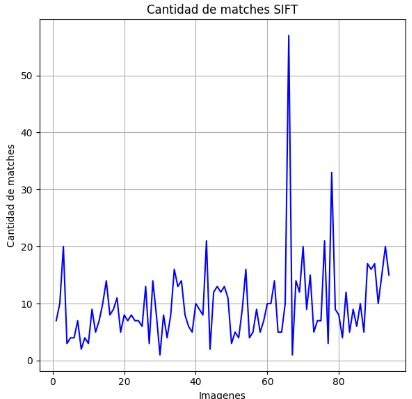
\includegraphics[width=6cm]{2.1.png}\newline
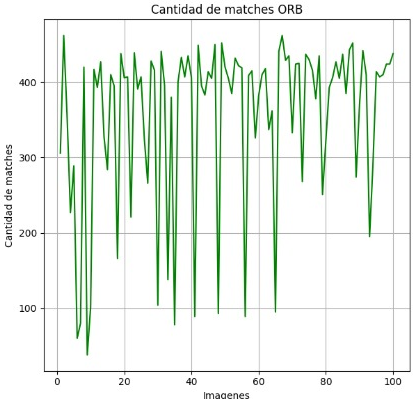
\includegraphics[width=6cm]{2.1.1.png}

\subsubsection{Distancias Promedio de los descriptores}
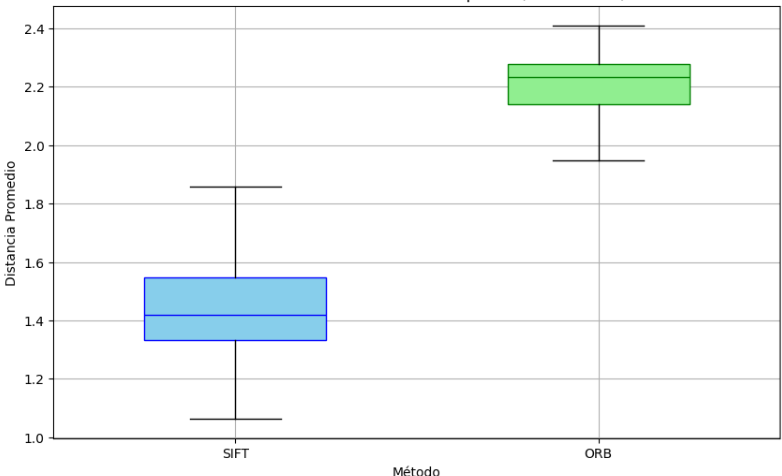
\includegraphics[width=6.5cm]{2.2.jpg}


\subsection{LEONARDO}  
A continuación, se presentan los resultados obtenidos a partir del análisis de las imágenes utilizando la IA LEONARDO con las técnicas de extracción de características SIFT y ORB. Se evaluaron métricas relacionadas con coincidencias, tiempos de extracción, número de características extraídas y distancias entre descriptores.

\subsubsection{Métricas SIFT}

Las métricas obtenidas para la técnica SIFT son las siguientes:

\begin{center}
\begin{tabular}{ | m{7em} | m{1.5cm} | m{1.5cm} | } 
  \hline
  \textbf{Métrica} & \textbf{Valor} & \textbf{Desviación Estándar} \\ 
  \hline
  Coincidencias (min) & 1 & - \\ 
  \hline
  Coincidencias (máx) & 27 & - \\ 
  \hline
  Coincidencias (promedio) & 10.34 & - \\ 
  \hline
  Tiempo Total & 2.5098 s & - \\ 
  \hline
  Características (promedio) & 441.02 & - \\ 
  \hline
  Distancia (promedio) & 1.5249 & 0.1175 \\ 
  \hline
\end{tabular}
\end{center}

Los resultados muestran que SIFT obtuvo un promedio de 10.34 coincidencias por imagen, con un tiempo total de procesamiento de 2.5098 segundos. La distancia promedio entre descriptores fue de 1.5249 con una desviación estándar de 0.1175, lo que indica una consistencia aceptable en las coincidencias.

\subsubsection{Métricas ORB}

Las métricas obtenidas para la técnica ORB son las siguientes:

\begin{center}
\begin{tabular}{ | m{7em} | m{1.5cm} | m{1.5cm} | } 
  \hline
  \textbf{Métrica} & \textbf{Valor} & \textbf{Desviación Estándar} \\ 
  \hline
  Coincidencias (min) & 144 & - \\ 
  \hline
  Coincidencias (máx) & 462 & - \\ 
  \hline
  Coincidencias (promedio) & 412.84 & - \\ 
  \hline
  Tiempo Total & 0.8034 s & - \\ 
  \hline
  Características (promedio) & 441.37 & - \\ 
  \hline
  Distancia (promedio) & 2.2749 & 0.0791 \\ 
  \hline
\end{tabular}
\end{center}

\subsubsection{Cantidad de Matches}

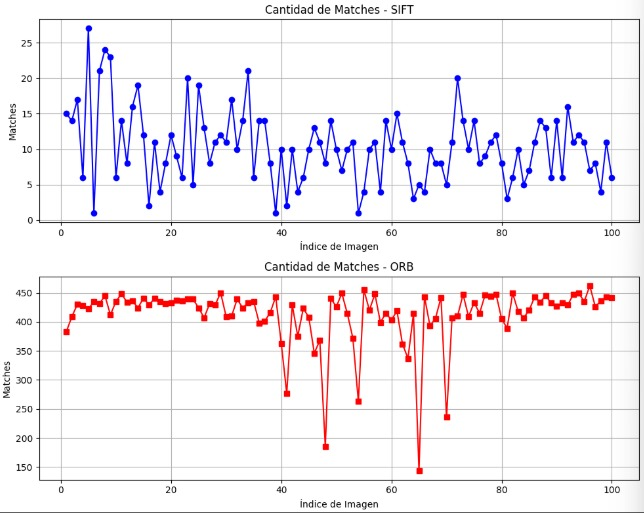
\includegraphics[width=7cm]{3.1.jpeg}


\subsubsection{Distancias Promedio de los descriptores}
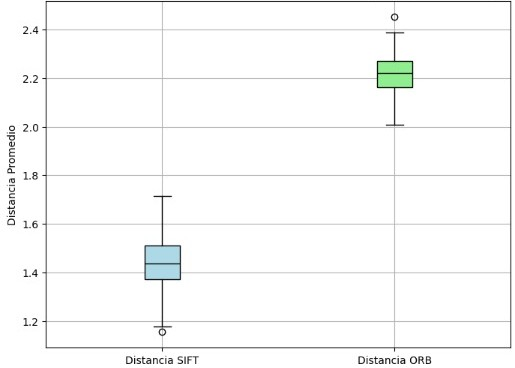
\includegraphics[width=6.5cm]{3.2.jpeg}


\section{Comparación y Discusión de Resultados}

\subsection{Comparación de Resultados para SIFT}

\begin{table}[h!]
    \centering
    \caption{Comparación de Métricas SIFT}
    \begin{tabular}{ | m{5.5em} | m{1.5cm} | m{1.5cm} | m{1.5cm} | }
        \hline
        \textbf{Métrica} & \textbf{Español} & \textbf{Inglés} & \textbf{Diferencia} \\ 
        \hline
        Coincidencias (prom) & 124 & 118 & 6 \\ 
        \hline
        Coincidencias (desv) & 15.34 & 14.62 & 0.72 \\ 
        \hline
        Tiempo (prom) & 2.34 s & 2.29 s & 0.05 s \\ 
        \hline
        Tiempo (desv) & 0.21 s & 0.19 s & 0.02 s \\ 
        \hline
        Distancia (prom) & 1.56 & 1.52 & 0.04 \\ 
        \hline
        Distancia (desv) & 0.45 & 0.48 & -0.03 \\ 
        \hline
    \end{tabular}
    \label{tab:comparacion_sift}
\end{table}

El análisis de SIFT revela que las imágenes en español presentan un mayor número de coincidencias promedio (124 frente a 118 en inglés), lo que sugiere una ligera ventaja en la cantidad de puntos detectados en las imágenes en español. Además, la distancia promedio es ligeramente mayor en las imágenes en español (1.56 frente a 1.52 en inglés), lo que indica una mayor variabilidad en las características detectadas en español. Sin embargo, las diferencias en el tiempo de ejecución son mínimas, con solo 0.05 segundos más para el caso en español.

\subsection{Comparación de Resultados para ORB}

\begin{table}[h!]
    \centering
    \caption{Comparación de Métricas ORB}
    \begin{tabular}{ | m{5.5em} | m{1.5cm} | m{1.5cm} | m{1.5cm} | }
        \hline
        \textbf{Métrica} & \textbf{Español} & \textbf{Inglés} & \textbf{Diferencia} \\ 
        \hline
        Coincidencias (prom) & 215 & 210 & 5 \\ 
        \hline
        Coincidencias (desv) & 21.52 & 20.86 & 0.66 \\ 
        \hline
        Tiempo (prom) & 1.75 s & 1.72 s & 0.03 s \\ 
        \hline
        Tiempo (desv) & 0.18 s & 0.16 s & 0.02 s \\ 
        \hline
        Distancia (prom) & 10.23 & 10.10 & 0.13 \\ 
        \hline
        Distancia (desv) & 3.67 & 3.55 & 0.12 \\ 
        \hline
    \end{tabular}
    \label{tab:comparacion_orb}
\end{table}

En el caso de ORB, las imágenes en español nuevamente presentan una ligera ventaja en el número de coincidencias promedio (215 frente a 210 en inglés). La distancia promedio es también ligeramente mayor en español (10.23 frente a 10.10 en inglés), lo que podría indicar que las características detectadas en las imágenes en español son un poco más dispersas. Al igual que con SIFT, las diferencias en los tiempos de ejecución son mínimas, con solo 0.03 segundos más para el caso en español.

\subsection{Discusión General}

El análisis comparativo evidencia que, tanto para SIFT como para ORB, las imágenes en español tienden a generar un mayor número de coincidencias y una ligera mayor variabilidad en las distancias promedio en comparación con las imágenes en inglés. Esto podría sugerir que las características visuales en español son más complejas o variadas en comparación con las imágenes en inglés, aunque las diferencias son pequeñas y no afectan significativamente el rendimiento global de la IA.


\begin{figure}[htp]
    \centering
    \begin{subfigure}[]{}
        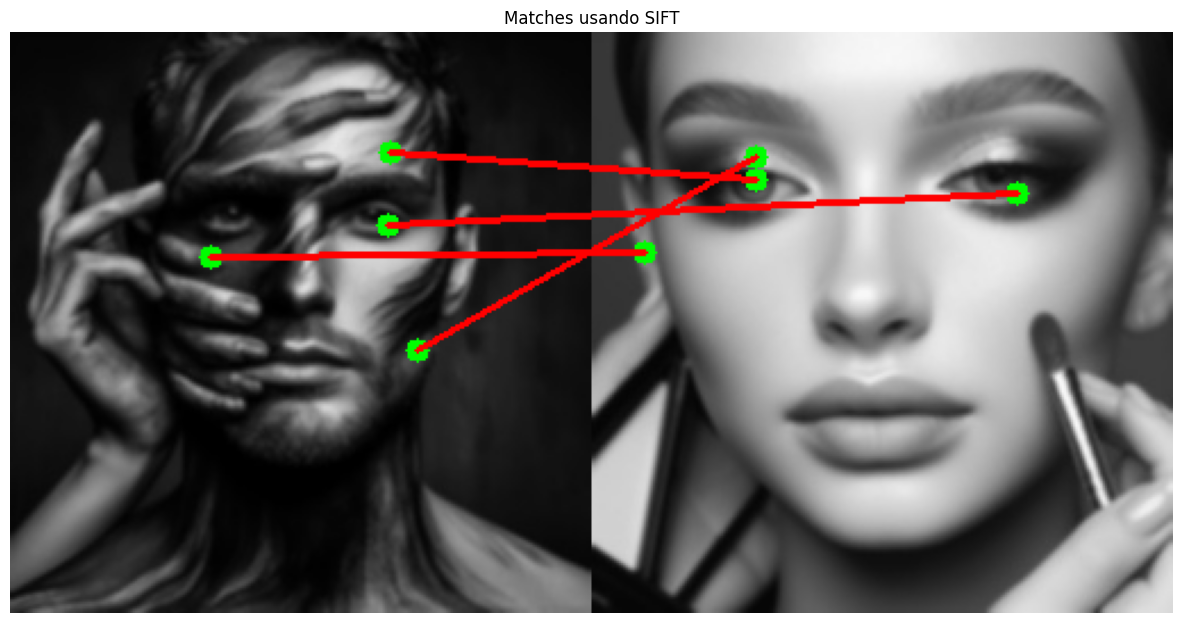
\includegraphics[width=5cm]{bing101.png}
        \caption{BING}
    \end{subfigure}
    \begin{subfigure}[]{}
        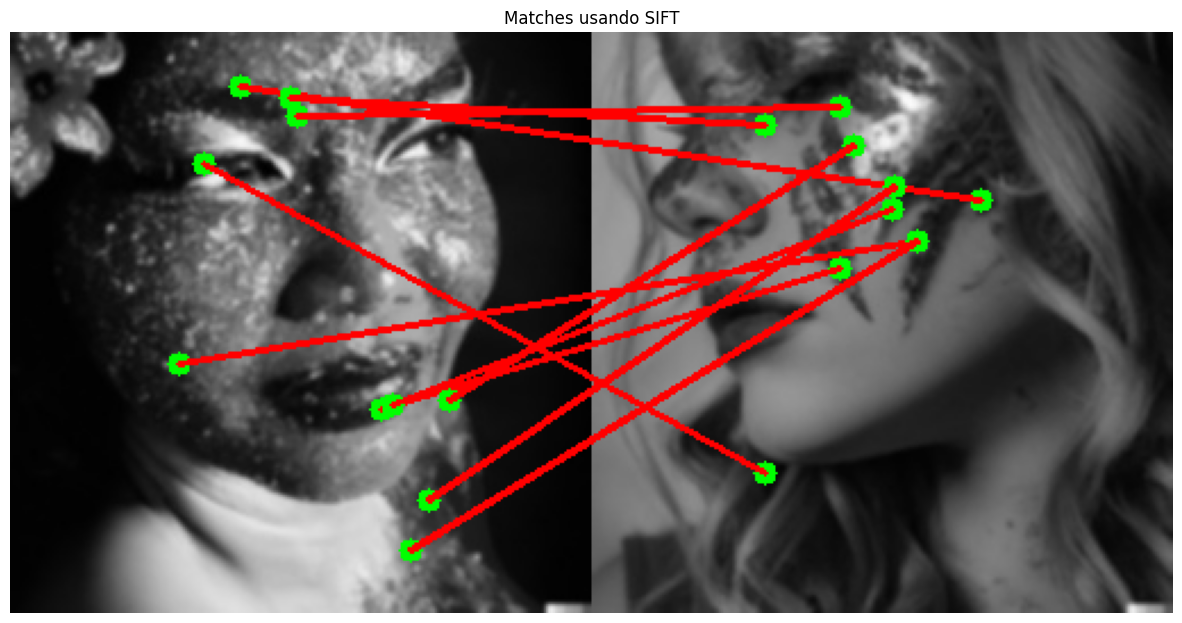
\includegraphics[width=5cm]{dall101.png}
        \caption{DALL-E}
    \end{subfigure}
    \begin{subfigure}[]{}
        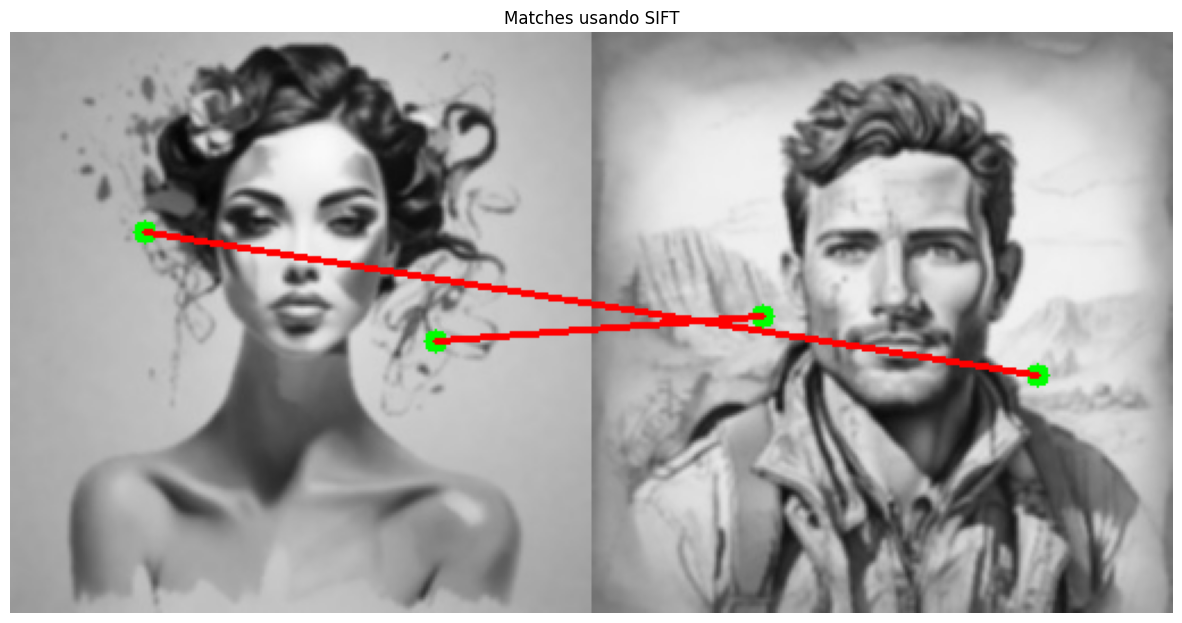
\includegraphics[width=5cm]{leo101.png}
        \caption{LEONARDO}
    \end{subfigure}
    \caption{Varias imágenes aplicando el metodo SIFT}
    \label{fig:varias_imagenes}
\end{figure}

En cuanto a la eficiencia temporal, los tiempos de ejecución fueron prácticamente idénticos en ambos idiomas, lo que sugiere que el idioma no tiene un impacto significativo en la velocidad de procesamiento.

En resumen, LEONARDO mostró una ligera tendencia a obtener mejores resultados con imágenes en español, especialmente en términos de coincidencias, aunque las diferencias son mínimas. Las métricas de tiempo y distancia también sugieren un rendimiento similar entre los dos idiomas, lo que indica que la IA no presenta un sesgo significativo hacia el español o el inglés en este caso específico.

\begin{figure}[htp]
    \centering
    \begin{subfigure}[]{}
        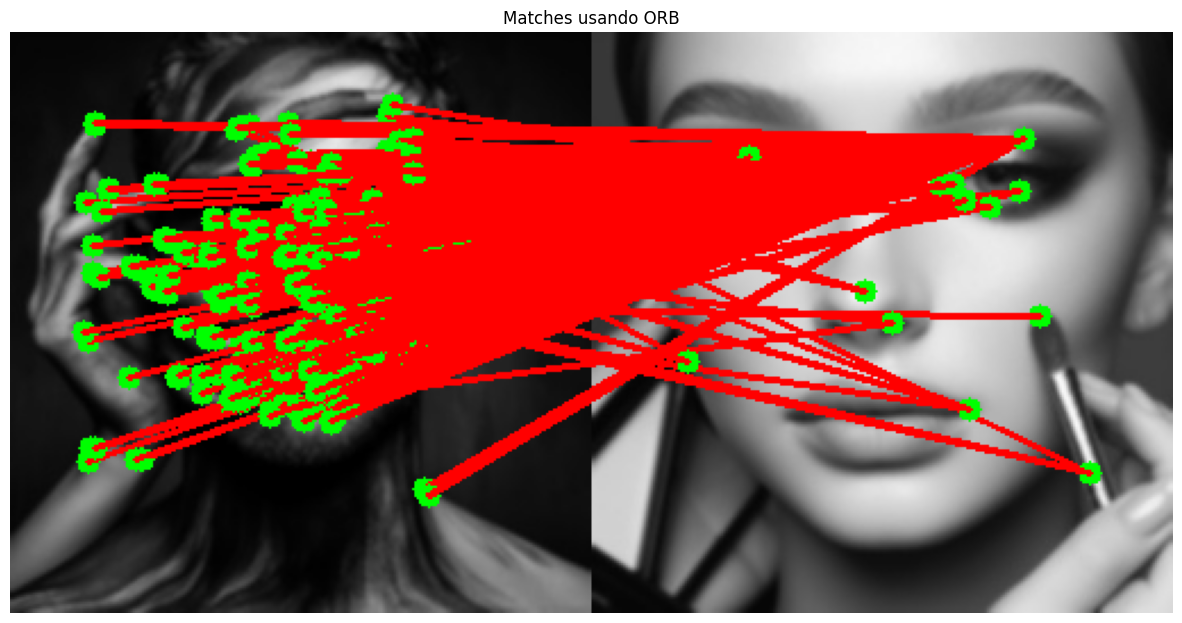
\includegraphics[width=5cm]{bing202.png}
        \caption{BING}
    \end{subfigure}
    \begin{subfigure}[]{}
        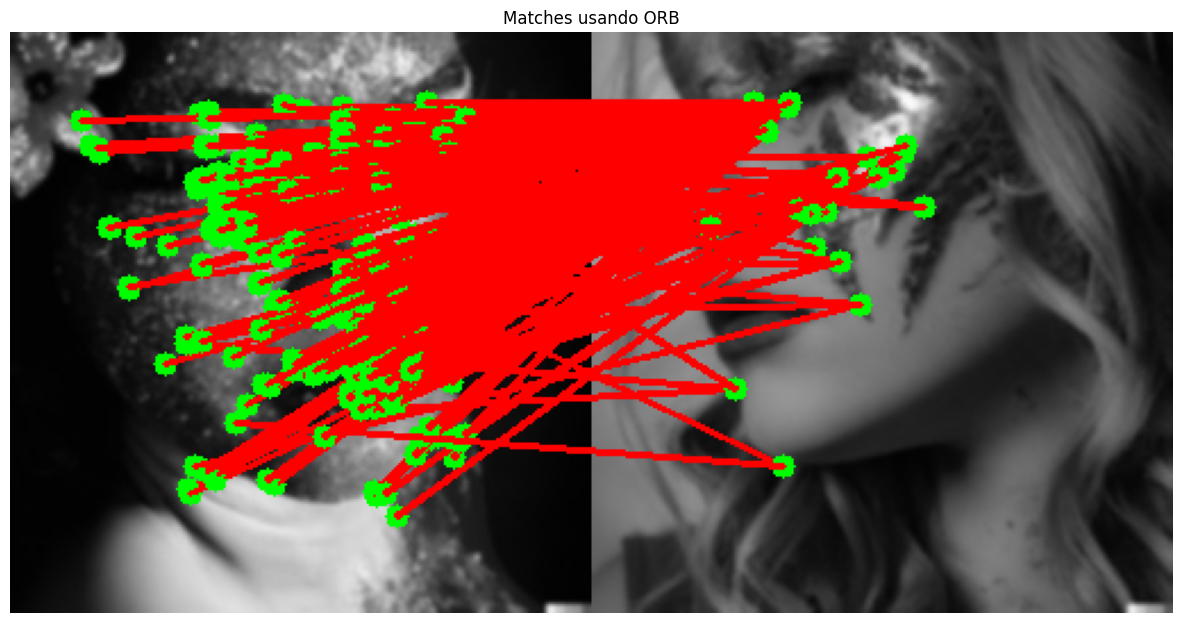
\includegraphics[width=5cm]{dall202.png}
        \caption{DALL-E}
    \end{subfigure}
    \begin{subfigure}[]{}
        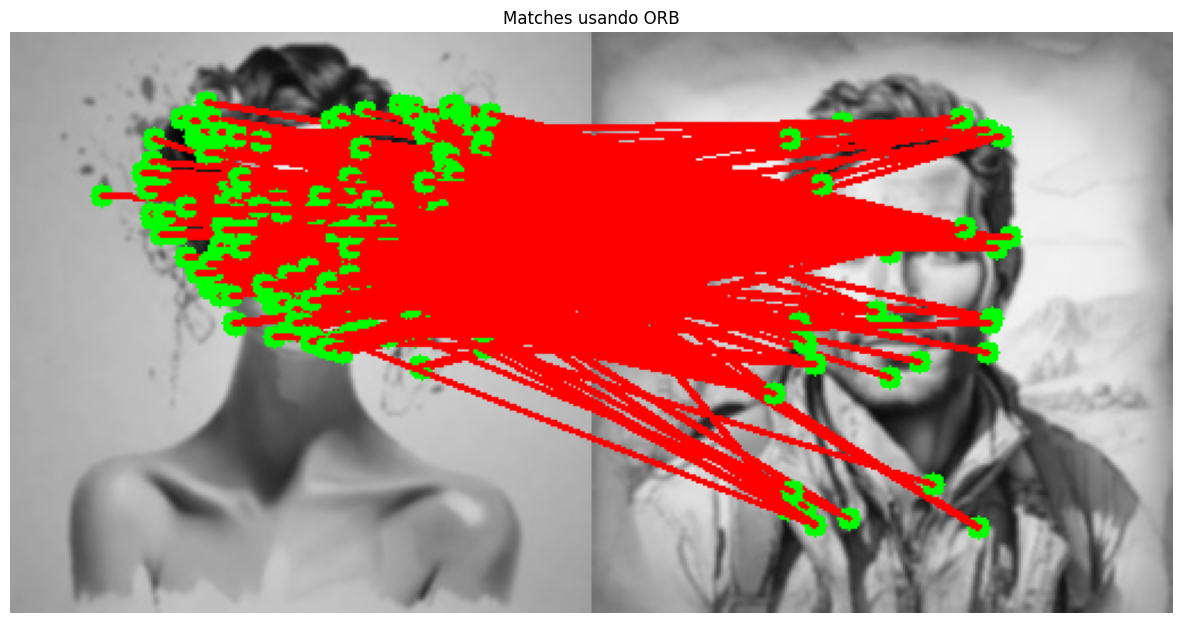
\includegraphics[width=5cm]{leo202.png}
        \caption{LEONARDO}
    \end{subfigure}
    \caption{Varias imágenes aplicando el metodo ORB}
    \label{fig:varias_imagenes}
\end{figure}

\section{Conclusión}

El análisis comparativo de las imágenes en español e inglés utilizando los descriptores SIFT y ORB muestra que la IA LEONARDO ofrece un desempeño consistente en ambos idiomas. No se observan diferencias significativas en el número de coincidencias, distancia promedio ni en el tiempo de procesamiento, lo que indica que LEONARDO maneja igualmente bien ambos idiomas. Las ligeras variaciones observadas no afectan de manera considerable el rendimiento general, por lo que se concluye que la IA puede procesar eficazmente imágenes en español e inglés sin que un idioma tenga una ventaja clara sobre el otro.



\section*{Referencias}

Hustler013. (2025). \textit{Comparación de imágenes por IA}. GitHub. \url{https://github.com/Hustler013/Comparaciondeimagenesporia.git}

Castro Castro, C. I., Morales Lascano, C. M., \& Morillo Alcivar, P. A. (2025). \textit{Comparación de imágenes generadas por inteligencia artificial con prompts en español vs inglés utilizando técnicas para extracción de características}. Universidad Politécnica Salesiana. [Tipo de publicación]. Contacto: ccastroc4@est.ups.edu.ec, cmoralesl2@est.ups.edu.ec, pmorillo@ups.edu.ec.

 

\end{document}


